The exponential distribution is memoryless, meaning that its distribution is the same regardless of how much time has passed. As the sojourn times, $S_S$, $S_{I_L}$ and $S_{I_H}$, are independent of each other and exponentially distributed, the expected time an individual will spend in a given state does not depend on how much time they already spent there or which states they visited earlier only the state they currently are in. Thus $\{X(t):t \geq 0 \}$  satisfies the Markov property
$$P(X(t+s)=j|X(s)=i, X(u), 0 \leq u \leq s)=P(X(t+s)=j|X(s)=j)$$ 
for $i,j = 0,1,...$ and for all $s \geq 0$ and $t >0 $.

%The jump probabilities are $P(S \rightarrow I_L)= 1 - \alpha$, $P(S \rightarrow I_H)= \alpha$, $P(I_L \rightarrow S)= P(I_H \rightarrow S) = 1$ and $P(I_L \rightarrow I_H)= P(I_H \rightarrow I_L) = 0$, since this is the probability to jump to a given state after the sojourn time ends.
%Using $\alpha = 0.10$, $P(S \rightarrow I_L)= 0.9$ and $P(S \rightarrow I_H)= 0.1$. 

%FORSLAG:
The jump probabilities are 
$$P(S \rightarrow I_L)= 1 - \alpha = 0.9 \quad P(S \rightarrow I_H)= \alpha = 0.1$$ 
%and 
$$P(I_L \rightarrow S)= P(I_H \rightarrow S) = 1 \quad P(I_L \rightarrow I_H)= P(I_H \rightarrow I_L) = 0,$$ 
since these are the probabilities to transition from one state to another after the sojourn time has ended.

%The transition rates are found from formula $q_{ij} = P(i \rightarrow j ) q_i$, where $q_i = \sum_{j \neq i} q_{ij}$. The rates are then expressed as $q_{SI_L} = (1-\alpha)\lambda $, $q_{SI_H} = \alpha \lambda$, $q_{I_LS} = 1/\mu_L$ and $q_{I_HS} = 1/\mu_H$. Using $\alpha = 0.10$ and inserting the values of $\lambda$, $\mu_L$ and $\mu_H$, the transition rates are 
%$$q_{SI_L} = 0.009,\text{ } q_{SI_H} = 0.001, \text{ } q_{I_LS} = 1/7, \text{ } q_{I_HS} = 1/20 \text{ and } q_{I_HI_L}=q_{I_LI_H}=0.$$

%FORSLAG: 
The transition rates can be found using the formula $q_{ij} = P(i \rightarrow j ) q_i$, where $q_i = \sum_{j \neq i} q_{ij}$, which results in
$$q_{SI_L} = (1-\alpha)\lambda = 0.009 \quad q_{SI_H} = \alpha \lambda = 0.001 \quad q_{I_LS} = \mu_L = \frac17  \quad q_{I_HS} = \mu_H = 0.05 $$
%and
$$ q_{I_HI_L}=q_{I_LI_H}=0. $$

This is illustrated in the transition diagram of $\{X(t):t \geq 0 \}$ in figure \ref{transdiagramA}.
%The transition diagram of $\{X(t):t \geq 0 \}$ is illustrated in figure \ref{transdiagramA}. 

\begin{figure}
    \centering
    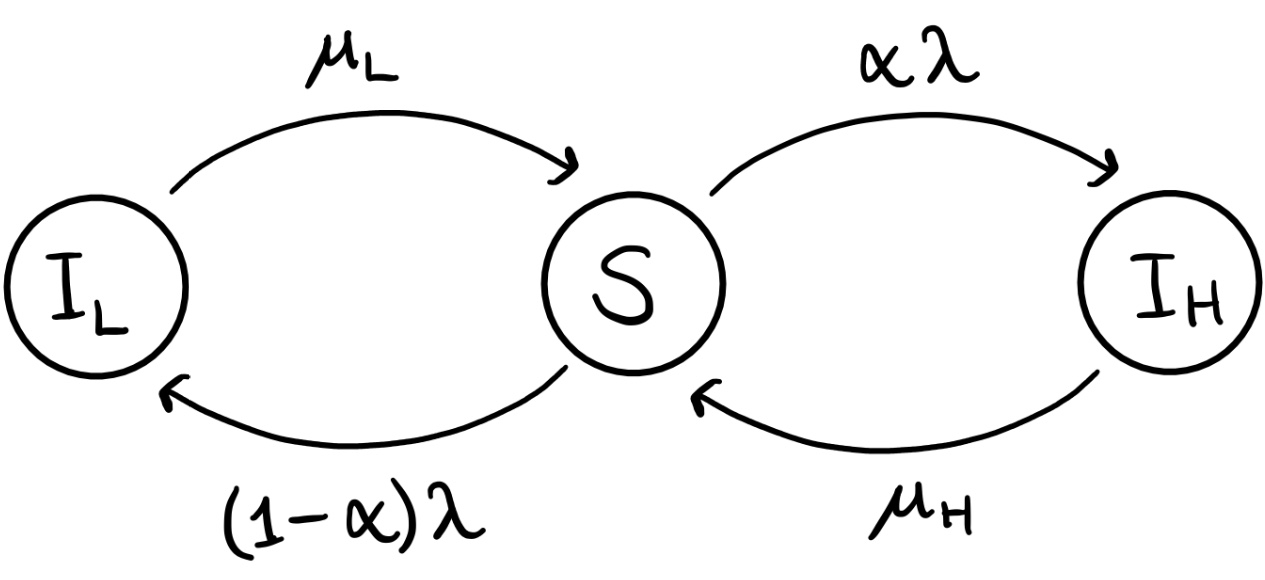
\includegraphics[width=80mm]{TransDiag1A.png}
    \caption{Transition diagram of $\{X(t):t\geq0\}$.}
    \label{transdiagramA}
\end{figure}




